\chapter{ADVENTURING AND EXPLORATION}

\begin{multicols}{2}

The player characters are typically pioneers and explorers struck with an insatiable wanderlust.  This section covers the inevitable situation when characters decide to travel into unfamiliar territory.

\section{TIME}

\index{Time}The passage of time in the game is based on the GM's choice.  He decides how time flows and how it is calculated in his game world.  Usually time will function exactly like it does in the real world: sixty seconds in a minute, sixty minutes in an hour, twenty-four hours equals a day, seven days to a week, four weeks to a month, and twelve months to a year.

Precise time in the game is measured in rounds and turns.  A round roughly equals a minute, although GMs can modify this.  A turn equals ten rounds or ten minutes.  Long-term time in the game, such as when days or weeks pass, can be skipped ahead if no important events occur.  Three weeks in game time can flash by in a minute of real time.

\section{MOVEMENT}

\index{Movement}The base movement values are listed by race.  The movement value represents the distance a character can move in a single round.  There are four kinds of movement available to characters.

\paragraph{Walking:} The standard walk represents characters moving through wide-open terrain like city streets or the wilderness.  Characters move at a brisk but steady pace and are readily aware of their surroundings.  Characters can walk a number of yards equal to their movement value multiplied by ten.

\paragraph{Cautious Walk:} Cautious movement is used in confined or hostile situations such as underground, in dungeons or buildings, or while fighting in combat.  Characters move slowly and steadily, watching for traps and enemies, and mentally mapping their surroundings.  Characters can cautiously walk a number of feet equal to their movement value multiplied by ten.

\paragraph{Hustle:} In situations where a cautious walk would be required, it's possible to hustle at the expense of awareness.  Characters can choose to move their standard walking movement value but suffer a $-1$ penalty to surprise rolls and a +1 bonus on opponent's surprise rolls.  Hustling characters cannot spot traps, secret doors, or other features that rely on careful study of the terrain.

\index{Running}\paragraph{Run:} When being chased, characters can choose to run to escape from their pursuers.  An initiative roll is made for the pursuers and escaping party.  If the fleeing party wins, they increase the distance from their pursuers by ten times the difference in feet or yards (depending on terrain and circumstance, as above).  The opposite is true if the pursuers win.  Like hustling, running characters suffer a penalty to surprise rolls and cannot spot hidden features.

\subsection{OVERLAND MOVEMENT}

\index{Overland Movement}A day's march lasts for 10 hours.  Under normal conditions, a character can walk twice his movement value in miles within 10 hours.  The slowest character sets the pace for the rest of the party.  Characters can force-march allowing them to cover two-and-a-half times their movement value in 10 hours, but at the end of a forced march, all characters must roll a constitution check (or a save vs. death for monsters or creatures with no known constitution score).  A $-1$ penalty to the check is applied for each consecutive day of forced marching.  Furthermore, forced marching applies a cumulative $-1$ penalty to attack rolls.  If the check fails, the character or party cannot force-march without resting for half a day per day spent forced marching.  Each half-day of rest also restores a lost point to attack rolls.  Characters can still continue overland travel at their normal movement value.  

\subsection{MOUNTED TRAVEL}

\index{Mounted Travel}A mounted rider can move his mount's movement value in miles within a day's march.  The slowest mount sets the pace for the rest of the group.  Mounts can be pushed to move double their movement value but must make a save vs. death with a cumulative $-1$ penalty for each day it was pushed.  On a failure, the mount can only move it's normal movement value until it receives at least one day of rest.  A mount can be forced to triple its movement value but must make a save vs. death at a $-3$ penalty or die from exhaustion.  If successful, the mount is exhausted and cannot be ridden for 1d3 days.

A mount that fails its save doesn't immediately collapse.  The GM decides where and when the mount becomes exhausted.

\subsection{TERRAIN AND VEHICLES}

\index{Vehicles}Vehicles with wheels, like a cart, are usually restricted to flat, open terrain. However, a wheeled vehicle could travel through rough terrain provided a good road is available.  Mountains and hills can be traversed slowly, but thick forests are impossible to navigate with a wheeled vehicle.  Dog sleds can only traverse snow or icy terrains and suffer no penalty to movement on them.  

\subsection{TERRAIN AND OVERLAND MOVEMENT}

Terrain can reduce or increase the distance traveled during overland movement.  First, figure the distance a character travels in a day's march (normally this is twice a character's movement value in miles).  This is the party's travel points for that day.  For each mile traveled in a specific terrain, subtract the listed cost from their travel points.  When travel points reach zero, the party has finished traveling for the day.

For example, a party with a movement value of 12 (24 miles per day) travels across grasslands for eight miles (8 travel points), low mountains for two miles (8 travel points), steep hills for one mile (4 travel points), and farmland for eight miles (4 travel points).  The low mountains and steep hills reduce their travel speed, but they pick up the pace on the farmlands for a total travel distance of 19 miles in that day's march.

\noindent
\begin{minipage}{\columnwidth}

\captionof{table}{Terrain Costs for Overland Movement}\label{overlandcosts}
\noindent
\begin{tabular}{|p{.7\columnwidth}|p{.2\columnwidth}|}
\hline
Terrain				& Cost \\
\hline\hline
\rowcolor[gray]{.9}Barren, wasteland	& 2 \\
Clear, farmland		& $^1$/$_2$ \\
\rowcolor[gray]{.9}Desert, rocky		& 2 \\
Desert, sand		& 3 \\
\rowcolor[gray]{.9}Forest, heavy		& 4 \\
Forest, light		& 2 \\
\rowcolor[gray]{.9}Forest, medium		& 3 \\
Glacier				& 2 \\
\rowcolor[gray]{.9}Hills, rolling		& 2 \\
Hills, steep		& 4 \\
\rowcolor[gray]{.9}Jungle, heavy		& 8 \\
Jungle, medium		& 6 \\
\rowcolor[gray]{.9}Marsh, swamp		& 8 \\
Moor				& 4 \\
\rowcolor[gray]{.9}Mountains, high		& 8 \\
Mountains, low		& 4 \\
\rowcolor[gray]{.9}Mountains, medium	& 6 \\
Grassland, plains	& 1 \\
\rowcolor[gray]{.9}Scrub, brush land	& 2 \\
Tundra				& 3 \\
\hline
\end{tabular}

\end{minipage}

\subsection{ROADS AND TRAILS}

\index{Roads and Trails}Vehicles cannot travel on terrain with a movement modifier greater than 1 unless there's a trail or road.  A trail is a cleared track, the result of natural movement normally along the path of least resistance.  Tracks reduce the movement modifier by half (1 becomes $^1$/$_2$, 4 becomes 2, and so on).  Clear plains or farmlands cannot be improved by a trail. 

Roads are rare and costly, usually existing only in areas with high traffic near cities or other centers of trade.  Roads in areas of level ground reduce the movement value to half-a-point per mile.  Roads reduce movement in mountainous terrain as a trail does.

\subsection{OBSTACLES AND HINDRANCES}

Normal movement assumes favorable conditions, but sometimes obstacles or hindrances can reduce movement speed.  Obstacles add to the movement value of the terrain they appear in.  Hindrances increase the terrain's movement value by the multiplier listed.

The modifiers for obstacles like chasms and cliffs assume there's a means to navigate around them.  If the traveling party doesn't encounter the obstacle in their path, it doesn't affect their movement value.  Extreme temperatures only affect a traveler if it's beyond their capability to withstand (for example, sweltering temperatures in a temperate region or a camel traveling in cold climes).  Streams and rivers don't modify movement if a bridge is available.

\noindent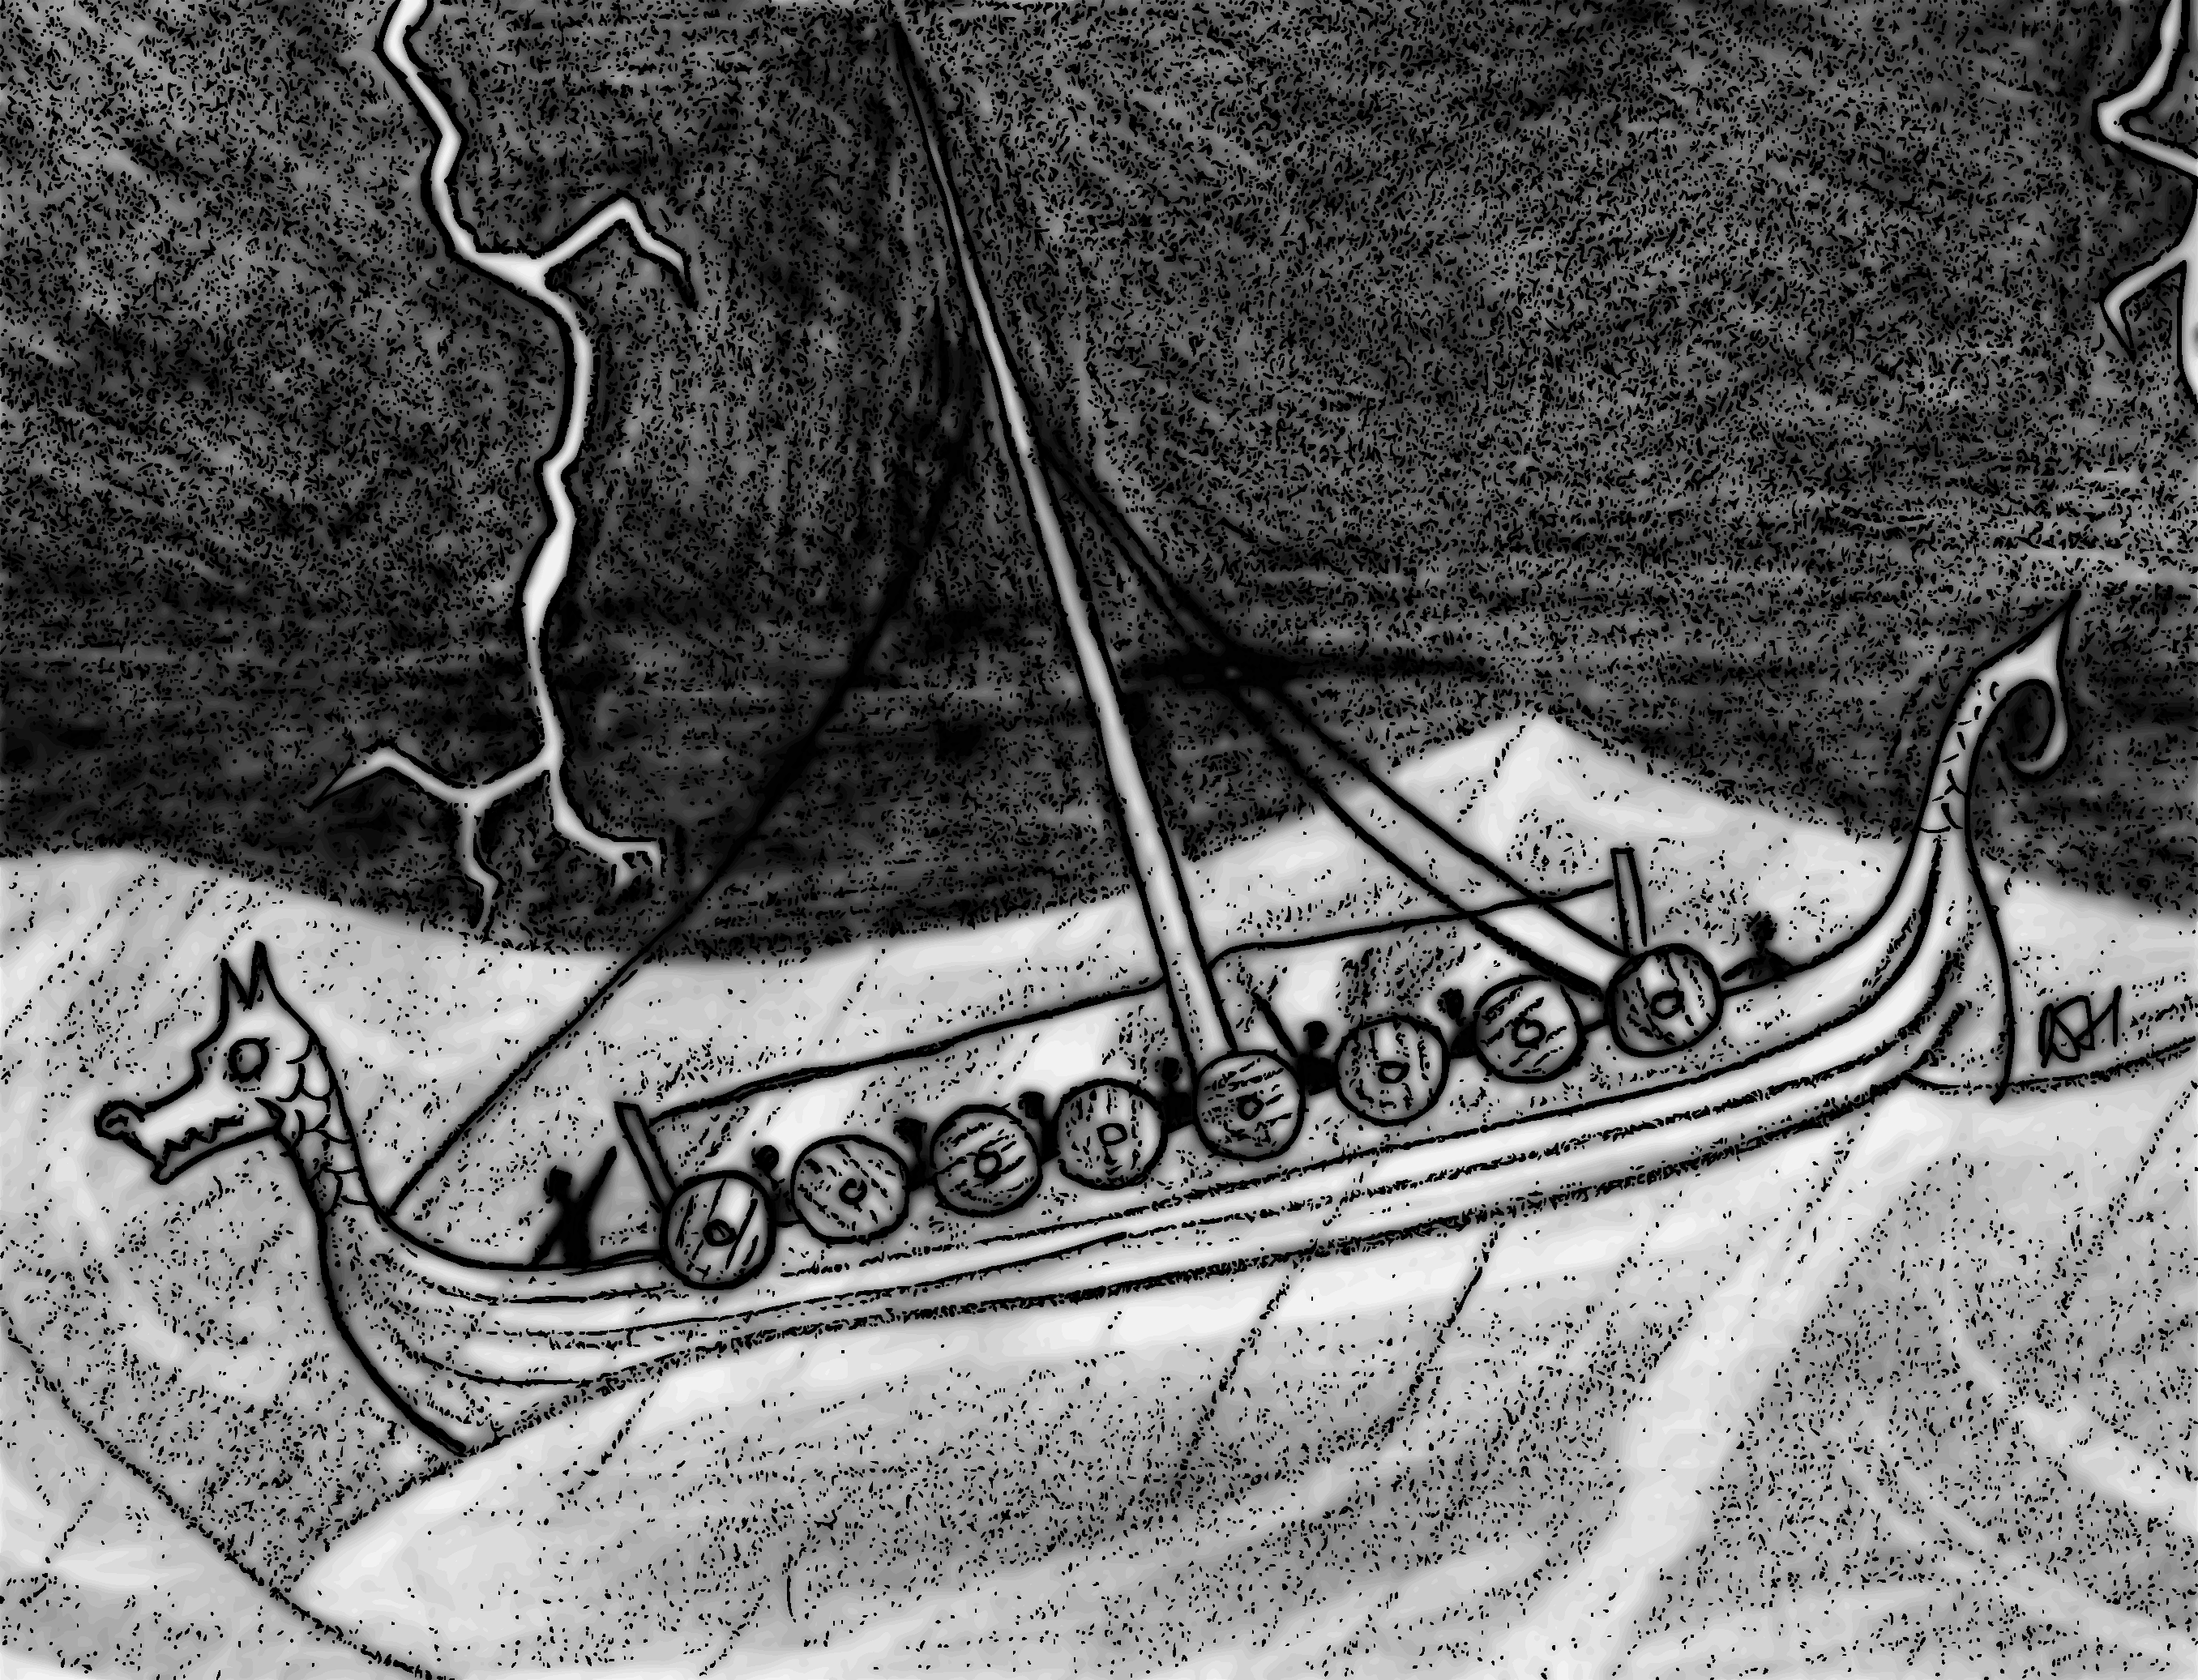
\includegraphics[width=\columnwidth]{vikingship.pdf}\label{vikingship}


\noindent
\begin{minipage}{\columnwidth}

\captionof{table}{Obstacles and Hindrances}\label{obstacles}
\noindent
\begin{tabular}{|p{.7\columnwidth}|p{.2\columnwidth}|}
\hline
Situation				& Modifier \\
\hline\hline
\rowcolor[gray]{.9}Chasm			& +3 \\
Cliff			& +3 \\
\rowcolor[gray]{.9}Dust/Sandstorm	& $\times$3 \\
Freezing		& +1 \\
\rowcolor[gray]{.9}Heavy wind		& +2 \\
Heavy fog		& +1 \\
\rowcolor[gray]{.9}Ice storm		& +2 \\
Mud				& $\times$2 \\
\rowcolor[gray]{.9}Rain, heavy		& $\times$2 \\
Rain, light		& +1 \\
\rowcolor[gray]{.9}Rain, torrential	& $\times$3 \\
Ravine			& +$^1$/$_2$ \\
\rowcolor[gray]{.9}Ridge			& +1 \\
River*			& +1 \\
\rowcolor[gray]{.9}Scorching		& +1 \\
Blizzard		& $\times$4 \\
\rowcolor[gray]{.9}Snow, normal	& $\times$2 \\
Stream			& +$^1$/$_2$ \\
\hline
\end{tabular}
\noindent\begin{tabular}{p{.95\columnwidth}}
*This modifier does not apply if a bridge is present. \\
\end{tabular}\vspace{.5em}

\end{minipage}

\section{WATER TRAVEL}

\index{Water Travel}There are two methods of traveling on water.  Each method assumes the proper craft, gear, and crew.

\subsection{RIVER}

The type of boat and the flow of the current determine movement value on a river.  When traveling downstream, the speed of the current is added to the speed of the boat.  When traveling upstream, the speed of the current is subtracted from the speed of the boat.  

Obstacles can be avoided when going upstream, but going downstream requires a good map or knowledgeable guide.  If placed in a harmful situation, the character piloting the craft must make a wisdom check to prevent capsizing.  Capsized boats are swept downstream and are destroyed by waterfalls or powerful rapids.

\subsection{OCEAN VOYAGE}

Ocean travel is primitive and dangerous.  Deep-sea sailing requires accurate instruments and an adequate crew.  Ships typically use sails but can be powered by oars.  Ships are rated based on their movement and seaworthiness.

\noindent
\begin{minipage}{\columnwidth}

\captionof{table}{Boat Movement}\label{boatmovement}
\noindent
\begin{tabular}{|p{.2\columnwidth}|p{.15\columnwidth}|p{.1\columnwidth}|p{.15\columnwidth}|p{.15\columnwidth}|}
\hline
Vessel	& Feet/ Round	& MPH	& Cargo	& Length \\
\hline\hline
\rowcolor[gray]{.9}Kayak			& 200	& 2		& 250 lbs.		& 8--10 ft. \\
Canoe, small	& 200	& 2		& 550 lbs.		& 10--15 ft. \\
\rowcolor[gray]{.9}Canoe, war		& 180	& 2		& 800 lbs.		& 25--35 ft. \\
Curragh			& 60	& 1*	& 600 lbs.		& 8--10 ft. \\
\rowcolor[gray]{.9}Keelboat, raft	& 60	& 1*	& 2,000 lbs.	& 15--20 ft. \\
Barge			& 60	& 1*	& 4,000 lbs.	& 25--40 ft. \\
\rowcolor[gray]{.9}Rowboat			& 160	& 1.5*	& 600 lbs.		& 8--12 ft. \\
\hline
\end{tabular}
\noindent\begin{tabular}{p{.95\columnwidth}}
*These vessels can triple their movement when the sail is raised and wind is favorable. \\
\end{tabular}\vspace{.5em}

\end{minipage}

A base mile per hour (MPH) is the distance a boat moves per hour.  If the number is separated by a slash, the first number is the sail speed and the second is the rowing speed.  Per round, a ship moves a number of yards equal to its MPH multiplied by 10.  Emergency move is the top speed a ship can move.  Emergency move strains the ship's resources severely and can only be sustained for a short amount of time before it starts to cause damage to the ship and her crew.  Seaworthiness is the chance a ship may sink during a dangerous situation like a storm, an extended voyage, being rammed, or an encounter with hidden obstacles.  If a d\% roll is higher than the seaworthiness rating, the ship sinks.  Anchored vessels have a +50\% bonus to their seaworthiness.

\noindent
\begin{minipage}{\columnwidth}

\captionof{table}{Ship Movement}\label{shipmovement}
\noindent
\begin{tabular}{|p{.25\columnwidth}|p{.1\columnwidth}|p{.2\columnwidth}|p{.25\columnwidth}|}
\hline
Ship	& MPH	& Emergency Move	& Seaworthiness \\
\hline\hline
\rowcolor[gray]{.9}Caravel		& 4		& 5		& 70\% \\
\rowcolor[gray]{.9}Coaster		& 3		& 4		& 50\% \\
Cog			& 3		& 4		& 65\% \\
\rowcolor[gray]{.9}Curragh		& 2/3	& 10	& 55\% \\
Drakkar		& 2/4	& 12	& 50\% \\
\rowcolor[gray]{.9}Dromond		& 2/9	& 12	& 40\% \\
Galleon		& 3		& 6		& 75\% \\
\rowcolor[gray]{.9}Great galley	& 3/6	& 11	& 45\% \\
Knarr		& 4/2	& 12	& 65\% \\
\rowcolor[gray]{.9}Longship	& 5/2	& 13	& 60\% \\
\hline
\end{tabular}

\end{minipage}

\subsection{WEATHER CONDITIONS}

\index{Weather}The weather can affect the movement value of ships.  Use the multipliers from the table to determine the final movement value of the ship. 

Weather is fairly consistent for the entire day.  The GM can decide the weather conditions for each day or roll for it randomly based on the current season.

Generally winds are favorable but sometimes can be adverse.  If winds are determined then roll 1d6; on a 5 or 6, the winds are adverse.  Adverse winds, storms and even worse weather blow a ship off course by half its movement modified by the wind ($\times$2 or more).

A strong wind applies a $-2$ penalty to all ranged attacks and affects movement.  Storms make it impossible to fire normal missiles and can knock creatures back.  Gale force winds make it impossible to fire any missile, including siege missiles, can uproot small trees, knock down weak structures, and endanger ships.  Hurricane force winds can destroy sturdier buildings and tear ships apart.

\noindent
\begin{minipage}{\columnwidth}

\captionof{table}{Weather Movement Modifiers for Ships}\label{weathershipmods}
\noindent
\begin{tabular}{|p{.27\columnwidth}|p{.3\columnwidth}|p{.28\columnwidth}|}
\hline
Weather			& Sailing Modifier	& Rowing Modifier \\
\hline\hline
\rowcolor[gray]{.9}Adverse			& $\times$$^1$/$_2$		& $\times$1 \\
Windless/Calm	& $\times$0*		& $\times$1 \\
\rowcolor[gray]{.9}Favorable wind	& 			&  \\
\rowcolor[gray]{.9}\hspace{2em}Average		& $\times$2		& $\times$1 \\
\hspace{2em}Strong		& $\times$3		& $\times$1** \\
\rowcolor[gray]{.9}Gale			& $\times$4**		& $\times$$^1$/$_2$** \\
Hurricane		& $\times$5***	& $\times$$^1$/$_2$*** \\
\rowcolor[gray]{.9}Light breeze	& $\times$1		& $\times$1 \\
Storm			& $\times$3**		& $\times$$^1$/$_2$** \\
\hline
\end{tabular}
\noindent\begin{tabular}{p{.95\columnwidth}}
*A ship cannot move using sails in calm winds or less. \\
**Seaworthiness check is required. \\
***Seaworthiness check at $-45$\% penalty is required. \\
\end{tabular}\vspace{.5em}

\end{minipage}

\noindent
\begin{minipage}{\columnwidth}

\captionof{table}{Random Wind}\label{randomwind}
\noindent
\begin{tabular}{|p{.05\columnwidth}|p{.25\columnwidth}|p{.25\columnwidth}|p{.25\columnwidth}|}
\hline
2d6	& Spring/Fall			& Summer			& Winter \\
\hline\hline
\rowcolor[gray]{.9}2	& Windless/calm		& Windless/calm		& Windless/calm \\
3	& Windless/calm		& Windless/calm		& Light breeze \\
\rowcolor[gray]{.9}4	& Light breeze		& Windless/calm		& Light breeze \\
5	& Moderate winds	& Light breeze		& Moderate winds \\
\rowcolor[gray]{.9}6	& Moderate winds	& Light breeze		& Strong winds \\
7	& Strong winds		& Moderate winds	& Strong winds \\
\rowcolor[gray]{.9}8	& Storm				& Moderate winds	& Storm \\
9	& Storm				& Strong winds		& Storm \\
\rowcolor[gray]{.9}10	& Gale				& Storm				& Gale \\
11	& Gale				& Gale				& Gale \\
\rowcolor[gray]{.9}12	& Hurricane*		& Hurricane*		& Hurricane* \\
\hline
\end{tabular}
\noindent\begin{tabular}{p{.95\textwidth}}
*Hurricanes occur only if the previous day's weather was gale.  Otherwise, treat hurricane as gale. \\
\end{tabular}\vspace{.5em}

\end{minipage}

\section{AERIAL MOVEMENT}

\index{Movement!Aerial}Aerial movement is handled under normal movement rules.  Weather modifies aerial movement and is essentially the sky's ``terrain."  Clear skies, with no more than moderate winds, are considered clear terrain for aerial movement.  The GM may choose the weather or determine it randomly.  To determine randomly, the GM rolls for wind conditions as above, using Table \ref{randomwind}.  If precipitation is not automatically indicated (such as storm, gale, etc.), the GM must roll 1d6.  In summer and winter, a roll of 6 on this die indicates rain or snow.  In spring and fall, a roll of 5 or 6 indicates rain.  Drier regions need not be checked, while wetter regions may have greater chance for precipitation.

Tiny flyers (the size of an eagle or smaller) are driven from the sky in a strong wind.  Man-sized flyers are buffeted out of the skies in gale force winds and large flyers cannot fly in storms.  Nothing can fly in a hurricane without magical protection.

The modifiers from this table are cumulative.  For example: gale force winds with rain applies a modifier of $^1$/$_2$~$\times$~$^1$/$_4$ = $^1$/$_8$, and strong winds with rain applies a modifier of $^1$/$_4$.

\noindent
\begin{minipage}{\columnwidth}

\captionof{table}{Aerial Movement Modifiers}\label{aerialmods}
\noindent
\begin{tabular}{|p{.45\columnwidth}|p{.45\columnwidth}|}
\hline
Condition		& Modifier \\
\hline\hline
\rowcolor[gray]{.9}Hurricane		& Impossible \\
Gale			& $\times$$^1$/$_4$ \\
\rowcolor[gray]{.9}Storm			& $\times$$^1$/$_4$ \\
Rain, snow		& $\times$$^1$/$_2$ \\
\rowcolor[gray]{.9}Strong wind		& $\times$$^1$/$_2$ \\
\hline
\end{tabular}

\end{minipage}

\subsection{Aerial Combat}

\index{Combat!Aerial}For the most part, aerial combat is treated the same as ground combat, with a few differences.  Most flyers (flying creatures, magical items and vehicles) cannot stop in place; they must keep moving forward to remain airborne, and since combat takes place in three dimensions, attacks can come from any direction, including above and below.  Aerial combat takes more game time.  Essentially, aerial combat consists of combatants maneuvering into position, taking dives and passes, and maneuvering back into a favorable position to attack again.  Rounds go by where combatants can do nothing except circle around, rolling initiative.  During these ``pass" rounds, combatants can escape, climb or dive as part of their movement.

The GM may treat flying movement values the same as ground movement. However, in purely aerial combat scenarios, precise distance measurements are not really necessary.   If using scale figurines, the GM may change the scale of the aerial battles and use the flying movement value as analogous to actual inches on a playing surface.  It is important to modify all combatants' movement values by any applicable weather or other modifiers before beginning the combat.

\paragraph{Altitude:} The GM must have a rough estimate of the number of feet of altitude at which the combatants are flying (see also Damage, Stalling, and Crashing).  It is assumed that most aerial combat is conducted at the same relative altitude; however, a flyer can attempt to change its altitude to gain a combat advantage.  For simplicity sake, while ascending (climbing) movement value is halved, and while descending (diving) movement value is doubled.  

A flyer above another can dive upon an opponent to gain a charge bonus to their attack.  During a successful dive attack, natural talons and claws as well as lances and spears cause double damage.  Flying creatures require natural weaponry and mounted flyers (including those using a fly spell, device or vehicle) require a large weapon to attack a flyer directly below them.  Because of the difficult angle, attacks made against a flyer directly above a flying combatant suffer a $-2$ penalty.

\index{Initiative!Flying}\paragraph{Initiative:} Flyers with better maneuver classes and better speed classes receive distinct advantages (see tables below).  At the beginning of combat, note the numerical values of the maneuver classes and speed classes of all combatants (ranging from 1 to 5).  The more agile combatant receives a bonus to his initiative rolls, between 0 and $-4$, equal to the difference between their maneuver class and the maneuver class of their opponent.  A 1-point bonus is also awarded to the faster opponent for every 2 points of difference between their speed classes, rounded up (maximum of $-2$ bonus when it's fast or god-like vs. slow).  Both bonuses may go to the same combatant for a total possible bonus of $-6$, or may be split between them.  Initiative is rolled (and modified) each round, whether any attacks occur during that round or not (Refer to Escaping, and see also Passes, Engagements and Dogfights).

\index{Speed Classes}\paragraph{Speed Class:} Flyers can be divided into 5 speed classes based upon their flying movement value.  A flyer can intentionally fly at a slower speed class, but unless this is expressly stated, speed class is always considered to be at the flyer's normal movement value.  Movement modifiers from diving or climbing do not affect the flyer's speed class.

\noindent
\begin{minipage}{\columnwidth}

\captionof{table}{Speed Classes}\label{speedclasses}
\noindent
\begin{tabular}{|p{.45\columnwidth}|p{.45\columnwidth}|}
\hline
Speed Class		& Movement Value \\
\hline\hline
\rowcolor[gray]{.9}1---Slow		& 12 or less \\
2---Average		& 13--24 \\
\rowcolor[gray]{.9}3---Quick		& 25--36 \\
4---Fast		& 37--48 \\
\rowcolor[gray]{.9}5---God-like*	& 49 or higher \\
\hline
\end{tabular}
\noindent\begin{tabular}{p{.95\textwidth}}
*God-like may include some hasted flyers. \\
\end{tabular}\vspace{.5em}

\end{minipage}

\index{Maneuver Classes}\paragraph{Maneuver Class:} Creatures, magical items and other vehicles that can fly will have a maneuver class listed alongside their movement value. Among other things, this value describes how tight of a turn the creature or object can make, ranging from 1---perfect (magical flight) to 5---clumsy (large, heavy fliers).   A flyer can intentionally fly with less agility, but unless this is expressly stated, maneuver class is always considered to be at the flyer's normal rating.

\noindent
\begin{minipage}{\columnwidth}

\captionof{table}{Maneuver Classes}\label{maneuverclasses}
\noindent
\begin{tabular}{|p{.18\columnwidth}|p{.08\columnwidth}|p{.22\columnwidth}|p{.08\columnwidth}|p{.19\columnwidth}|}
\hline
Maneuver Class 	& Turns	& Passes			& Hover & Momen\-tum \\
\hline\hline
\rowcolor[gray]{.9}1---Perfect		& 12	& Normal			& Yes 	& None \\
2---Good		& 6		& 1 per round		& Yes		& None \\
\rowcolor[gray]{.9}3---Average		& 3		& 1 per 2 rounds	& No		& $^1$/$_2$ Move \\
4---Poor		& 2		& 1 per 3 rounds	& No	& $^1$/$_2$ Move \\
\rowcolor[gray]{.9}5---Clumsy		& 1		& 1 per 6 rounds	& No		& $^1$/$_2$ Move \\
\hline
\end{tabular}

\end{minipage}

\paragraph{Hover:} Perfect and good flyers can hover.  Flyers that can hover don't have to maintain momentum each round.  This allows them to maintain their altitude, or climb and dive without moving forward.

\paragraph{Momentum:} Indicates the minimum distance a flyer must travel during a round.  With the exception of perfect and good flyers, all other creatures must maintain forward momentum or else they stall in the air and fall.  Momentum can be maintained in any direction and a flyer can turn if they wish.  For example, a flyer with average maneuver class and a movement value of 12 must fly at least 6 and can make up to 3 turns while doing so.

\paragraph{Turns:} Flyers are limited to the number of direction changes (or turns) they can make in a single round.  In general, a single turn is a 30-degree angle, and 12 turns equal 360 degrees (a full circle).

\paragraph{Passes, Engagements and Dogfights:} Aerial combat is concerned with two things: maneuver class and speed class.  Unlike ground combat, aerial combat is about positioning and maneuvering.  Attackers position themselves to catch up with and strike their opponents who are likewise trying to evade attacks and intercept them.  Fast, agile flyers always have an advantage over slow, clumsier flyers.  

Passes represent the number of rounds it takes for a flyer to perform one melee or non-magical ranged attack (such as a breath weapon) upon a relatively stationary opponent.  Stationary opponents include those on the ground, those using a \textit{levitate} spell (or hovering in place) and those flyers with the same speed class as the attacker.  Passes can also represent the nature of aerial combat where flyers must break off, reposition, and then prepare for another attack, but this abstraction can be ignored if miniatures and scale measurements are used.

In aerial combat, the combatants will engage each other as they do in ground combat and enter a dogfight.  In addition to the initiative bonuses given to faster and more maneuverable flyers, the number of rounds between attacks can be increased or decreased based on the relative speed class.  Add or subtract the difference between the opponents' speed classes to the number of rounds per attack.  Only perfect flyers are able to treat aerial combat the same as ground combat.  They can attack their normal number of times each round, unless their opponent is faster.   All other maneuver classes are limited to 1 attack per round, regardless of bonuses.
 
In the following examples, MC is Maneuver Class and SC is Speed Class.
 
\paragraph{Example 1:} A flyer with an MC5/SC3 (clumsy but quick) versus a flyer with an MC3/SC1 (average and slow).  If the speed classes had been equal, the flyer with MC5 would attack once every six rounds, and the flyer with MC3 would attack once every two rounds, but there is a 2-point difference in speed class.  So, the flyer with MC5 would attack once per four rounds (6~$-$~2 = 4), and the flyer with MC3 would also attack once every four rounds (2~+~2 = 4).  The speed difference put them on even footing.
 
\paragraph{Example 2:} MC5/SC1 (clumsy and slow) vs. MC3/SC3 (average and quick).  MC5 would attack 1/8 rounds and the MC3 would attack once every round (the maximum).

\paragraph{Example 3:} MC5/SC1 (clumsy and slow) vs. MC2/SC5 (good and godlike).  There is now a 4-point difference, so MC5 would attack 1/10 rounds and MC2 still attacks only once per round.

\paragraph{Example 4:} MC5/SC5 (clumsy but godlike) vs. MC2/SC1 (good but slow).  MC5 attacks 1/2 rounds, due to its god-like speed, while MC2 is reduced to only 1/5 rounds.
 
\paragraph{Example 5:} MC5/SC1 (clumsy and slow) vs. MC1/SC4 (perfect and fast). MC5 attacks 1/9 rounds and MC1 gets its normal attacks each round (no change).
 
\paragraph{Example 6:} MC5/SC4 (clumsy but fast) vs. MC1/SC1 (perfect but slow).  MC5 attacks 1/3 rounds and MC1 is reduced to 1 normal attack every 4 rounds.

\paragraph{Escaping:} A flyer that is both faster and more maneuverable than its opponent can break off and escape during its initiative, with no free attack against it.  A flyer that is faster but equally or less maneuverable can escape during their initiative, but suffers the free attack against it.  A flyer that is slower but more maneuverable, must win the initiative roll to escape without a free attack against it, but can escape during a lost initiative by accepting a free attack against it.   A flyer that is slower and equally or less maneuverable than its opponent must win the initiative roll to escape, but still suffers the free attack against it.  Ground based opponents may attempt to escape normally.

\paragraph{Breath Weapons \& Spells:} It's easier to employ a breath weapon or cast a spell with an effective area on the ground than it is in the air.  When using a breath weapon, a 60-degree arc in front of the creature is the blast area.  When a spell with an effective area is cast, the blast area is half the size of the effective area starting from the center.  Creatures inside the blast area roll normal saving throws.  Any creatures caught inside the effective area, but outside the blast area, receive a +2 bonus to applicable saves.

\paragraph{Missile Fire:} Mounted flyers that are in motion (including those using a \textit{fly} spell, a device or vehicle), suffer the same penalty while firing a ranged weapon as if they were mounted on the ground.  A hovering creature, even if mounted or using a \textit{fly} spell, doesn't suffer this penalty.
 
\paragraph{Damage, Stalling, and Crashing:} With the exception of perfect flyers, those that sustain damage equal to or greater than 50\% of their maximum hit points are reduced to half movement value and must immediately land.  These flyers can usually glide safely to the ground but cannot climb until healed to above 50\%.  Good flyers also lose their ability to hover until healed to above 50\%.  If the GM determines that no safe landing spot is available, the result is a crash landing.  The GM must adjudicate crash landings based on factors, such as the altitude and ground terrain, as well as the speed, size and type of flyer, but the damage should be no less than 2d6 and no more than 10d6. 

In general, the faster a flyer is moving when it crashes, the more damage it takes.  If a flyer strikes a solid object in mid-air, it crashes, suffering damage equal to 2d6 per its current speed class (10d6 maximum).  A flyer that has crashed into an obstacle immediately stalls and falls.  Flyers that stall in mid-air (see also Momentum), or those whose fly spell suddenly ends, fall straight down a number of feet equal to five times their momentum requirement.  A flyer that hits the ground before the end of the fall crashes; taking 1d6 damage per current speed class (1--5) for every 10 feet of fall completed.  The minimum damage is 2d6 and the maximum damage is 20d6.  A stalled flyer that doesn't crash by the end of its fall, assuming it is still conscious and less than 50\% damaged, can regain its composure and begin to fly normally again.  The faster the flyer is moving when it stalls the farther it falls. For this reason, fast flyers (movement value of 48) prefer combat at altitudes in excess of 120 feet (48~$\div$~2 = 24~$\times$~5 = 120').  Slower flyers (movement value of 12) often attempt to conduct combat at lower altitudes of 30 feet (12~$\div$~2 = 6~$\times$~5 = 30') or around tree top level, to discourage a faster opponent from taking full advantage of its speed.

\section{BECOMING LOST}

\index{Becoming Lost}It's possible to become lost while traveling.  Characters are either lost or hopelessly lost.

\subsection{LOST}

Becoming lost occurs when the travelers don't know the route to their destination but know how to return to the starting point.  Finding the right direction or returning to the starting point is simply a matter of time.  This generally occurs when following unfamiliar paths or poorly marked trails, or when consulting poorly drawn maps or badly worded directions.  Becoming lost is a setback but is rarely dangerous.

\subsection{HOPELESSLY LOST}

Becoming hopelessly lost happens when characters don't know where they are, which way to go, or how to get back where they started.  A check should be made whenever the characters move overland without following a road, river, or well-traveled trail, and whenever a river they are following empties into a swamp, estuary, or delta.  One check should be made each day these conditions persist.  If the die roll is less than the modified percentage, the characters are hopelessly lost.

If a party is hopelessly lost, they make no further checks until they find a way to regain their bearings (they get directions, find a road, etc.).  The GM should refrain from telling players that their characters are lost.  The GM should randomly determine the general direction the party travels per day while they're lost by rolling 1d8; 1 is north, 2 is north-east, 3 is east, 4 is south-east, 5 is south, 6 is south-west, 7 is west, 8 is north-west.

\noindent
\begin{minipage}{\columnwidth}

\captionof{table}{Chance of Becoming Hopelessly Lost}\label{lostchance}
\noindent
\begin{tabular}{|p{.7\columnwidth}|p{.2\columnwidth}|}
\hline
Surroundings			& \% Chance \\
\hline\hline
\rowcolor[gray]{.9}Level, open ground		& 10\% \\
Rolling ground			& 20\% \\
\rowcolor[gray]{.9}Lightly wooded			& 30\% \\
Rough, wooded and hilly	& 40\% \\
\rowcolor[gray]{.9}Swamp					& 60\% \\
Mountainous				& 50\% \\
\rowcolor[gray]{.9}Open sea				& 20\% \\
Thick forest			& 70\% \\
\rowcolor[gray]{.9}Jungle					& 80\% \\
\hline
\end{tabular}

\end{minipage}

\noindent
\begin{minipage}{\columnwidth}

\captionof{table}{Lost Modifiers}\label{lostmods}
\noindent
\begin{tabular}{|p{.7\columnwidth}|p{.2\columnwidth}|}
\hline
Condition				& Modifier \\
\hline\hline
\rowcolor[gray]{.9}No landmarks*			& +50\% \\
Darkness				& +70\% \\
\rowcolor[gray]{.9}Overcast				& +30\% \\
Navigator with group	& $-30$\% \\
\rowcolor[gray]{.9}Landmark sighted		& $-15$\% \\
Local guide				& Variable** \\
\rowcolor[gray]{.9}Poor trail				& $-10$\% \\
Raining					& +10\% \\
\rowcolor[gray]{.9}Directions, map, tools	& Variable** \\
Fog or mist				& +30\% \\
\hline
\end{tabular}
\noindent\begin{tabular}{p{.95\columnwidth}}
*Includes sailing out to sea beyond sight of land. \\
**GM decides usefulness of guide or directions. Generally, more expensive guides or maps are more useful. \\
\end{tabular}\vspace{.5em}

\end{minipage}

\section{SWIMMING}

\index{Swimming}Swimming is a skill that a character can learn.  Characters are capable of swimming a number of yards in a single round equal to half their movement value multiplied by 10.  Swimmers can gain a burst of speed, thus moving their full movement value in a single round, by rolling a strength check against half their strength score (exceptional strength counts as 9).  \index{Armor!Effects on Swimming}Characters wearing metal armor instantly sink to the bottom; however, they can walk along the bottom at $^1$/$_3$ their movement value.  

\index{Constitution!and Swimming}A character can normally swim (at half speed) for a number of hours equal to his constitution score.  A constitution check (or a save vs. death if no constitution score is known) must be made for each additional hour of swimming.  If a swimmer fails this constitution check, he must tread water for half an hour before he can continue swimming (this time counts as time spent swimming).  Furthermore, additional hours spent swimming reduces constitution by 1 point temporarily and applies a cumulative penalty of $-1$ to all attack rolls.  A character drowns if his constitution score drops to 0 while swimming.  

Normal travel assumes swimming in calm waters.  Choppy water or swimming against the tide requires a constitution check every hour of swimming.  Rough water or swimming against a heavy tide requires a constitution check every half hour.  Stormy water requires a constitution check every round.  The GM may modify the constitution points lost in rougher waters.

Characters can swim fast for longer distances but at an increased risk.  A swimmer can move at his full movement value but he must make a constitution check every hour, his strength and constitution are reduced by 1 point every hour, and a cumulative $-2$ penalty to his attack rolls is applied every hour.  Characters can swim twice their movement value but must roll a constitution check every turn, and the penalties are accrued every turn spent swimming.  Drowning occurs when either strength or constitution reaches 0.

Characters can recover lost ability score points and attack penalties by resting.  Each day of rest recovers 1d6 ability points (1d3 points for strength and constitution if swimming at a hustle) and restores 2d6 points worth of attack penalties.  

\subsection{HOLDING A CHARACTER'S BREATH}

\index{Holding One's Breath}If able to get a gulp of air in advance, characters can hold their breath for a number of rounds equal to $^1$/$_3$ their constitution score (round up).  If characters exert themselves (moving more than half their movement value, fighting, or swimming in rough water), this time is halved (rounded up).  Characters in metal armor are considered to be exerting themselves.  If unable to get a gulp of air, these times are reduced by half.  All characters are capable of holding their breath for at least one round regardless of circumstances.  Holding one's breath beyond this time requires a constitution check each round.  Each subsequent check suffers a -2 cumulative penalty.  On a failed check, the character must breathe.  If he cannot breathe then he drowns.

\index{Swimming!Diving}\index{Diving}\paragraph{Diving:} Regardless of movement, swimmers can swim downwards 20 feet in a single round.  A brief run or jumping several feet above the water adds 10 feet of depth to the initial dive.   For every 10 feet of height above the water an additional 5 feet of depth can be added up to a maximum of 20 additional feet.  By contrast, if prepared for shallow water, a character can dive from a height of up to 50 feet without being injured, as long as the water is at least 3-feet deep per 10 feet of the height of the dive.  

\paragraph{Surfacing:} Regardless of movement, swimmers can rise at the rate of 20 feet per round.  Characters floating to the surface (such as dead or unconscious characters) rise at a rate of 5 feet per round.
 
\subsection{VISION UNDERWATER}

\index{Vision!Underwater}Under normal conditions (bright sunlight), vision extends out to 50' in freshwater and 100' in saltwater.  For every 10' below the surface, vision is reduced by 10' until it becomes pitch black.  On overcast days, normal vision underwater is reduced to half, and characters cannot see at all on moonless nights.  Artificial light sources, such as magic, only illuminate half their normal area underwater.

\section{CLIMBING}

\index{Climbing}Climbing is a general skill anyone can learn.  For most characters, climbing requires specialized equipment such as ropes and pitons.  Only thieves can climb without the use of equipment.  A climb check is made whenever a character attempts to ascend more than 10 feet.  The base climb check is 40\% modified by special conditions.  Thieves use their climb walls rate to climb.  The climb check is made before the character begins climbing.  If the check is successful, the character need not make a new check unless conditions worsen.  If the character fails their initial climb check they find no means of climbing and cannot even begin.  A character may retry a failed climb check only if conditions would improve their check or they find a suitable location at least half-a-mile away.

\noindent
\begin{minipage}{\columnwidth}

\captionof{table}{Climbing Modifiers}\label{climbingmods}
\noindent
\begin{tabular}{|p{.7\columnwidth}|p{.2\columnwidth}|}
\hline
Situation								& Modifier \\
\hline\hline
\rowcolor[gray]{.9}Prominent handholds (branches, ledges)	& +40\% \\
Rope and wall							& +55\% \\
\rowcolor[gray]{.9}Sloped inward							& +25\% \\
Armor									& \\
\hspace{2em}Banded, splint						& -25\% \\
\rowcolor[gray]{.9}\hspace{2em}Plate									& -50\% \\
\hspace{2em}Scale, chain							& -15\% \\
\rowcolor[gray]{.9}\hspace{2em}Studded leather, padded				& -5\% \\
Character race*							& \\
\hspace{2em}Dwarf									& -10\% \\
\rowcolor[gray]{.9}\hspace{2em}Gnome									& -15\% \\
\hspace{2em}Halfling								& -15\% \\
\rowcolor[gray]{.9}Encumbrance**							& -5\% \\
Surface condition						& \\
\hspace{2em}Slightly slippery (wet/ crumbling)	& -25\% \\
\rowcolor[gray]{.9}\hspace{2em}Slippery (icy/ slimy)					& -40\% \\
Climber $^1$/$_2$ HP or less			& -10\% \\
\hline
\end{tabular}
\noindent\begin{tabular}{p{.95\columnwidth}}
*Same modifiers listed for thieves. Do not apply twice. \\
**This penalty is cumulative for each point a character's speed is reduced below their base. \\
\end{tabular}\vspace{.5em}

\end{minipage}

\subsection{CLIMB SPEED}

\index{Climbing Speed}Climb speed is determined by the surface a character is climbing on.  All characters are able to climb their movement value in feet, multiplied based on the type of surface, in one direction (up, down, sideways, or diagonal) per round.  Thieves climb at double the speed of a normal character and their speed modifiers are listed in brackets [\#].

Climbing characters cannot use items requiring two hands, unless they find secure footing.  If struck while climbing, regardless of damage, a climb check must be made immediately to maintain hold.  If a roped character fails, he must spend a round to regain his handhold.  An un-roped character falls on a failure.

\noindent
\begin{minipage}{\columnwidth}

\captionof{table}{Climbing Speed Modifiers}\label{climbinbspeedmods}
\noindent
\begin{tabular}{|p{.35\columnwidth}|p{.15\columnwidth}|p{.15\columnwidth}|p{.15\columnwidth}|}
\hline
Surface				& Dry					& Slightly Slippery		& Slippery \\
\hline\hline
\rowcolor[gray]{.9}Very smooth*		& $^1$/$_4$ [$^1$/$_2$]	& -- [$^1$/$_4$]		& --** \\
Smooth, cracked*	& $^1$/$_2$ [1]			& $^1$/$_3$ [$^2$/$_3$] & $^1$/$_4$ [$^1$/$_2$] \\
\rowcolor[gray]{.9}Rough*				& 1 [2]					& $^1$/$_3$ [$^2$/$_3$]	& $^1$/$_4$ [$^1$/$_2$] \\
Rough w/ledges		& 1 [2]					& $^1$/$_2$ [1]			& $^1$/$_3$ [$^2$/$_3$] \\
\rowcolor[gray]{.9}Ice wall			& --					& --					& $^1$/$_4$ [$^1$/$_2$] \\
Tree				& 4 [8]					& 3 [6]					& 2 [4] \\
\rowcolor[gray]{.9}Sloping wall		& 3 [6]					& 2 [4]					& 1 [2] \\
Rope and wall		& 2 [4]					& 1 [2]					& $^1$/$_2$ [1] \\
\hline
\end{tabular}
\noindent\begin{tabular}{p{.95\columnwidth}}
*Non-thieves require climbing gear to climb these surfaces. \\
**It is impossible to climb very smooth, slippery surfaces with mundane tools. \\
\end{tabular}\vspace{.5em}

\end{minipage}

\subsection{CLIMBING TOOLS}
\index{Climbing!Climbing Tools}The basic tools for climbing are pitons (spikes), ropes, and ice axes.  Tools do not actually aid in climbing; rather, they prevent falling.  A character can only fall as far as their rope or twice the distance to the last piton they placed.  Pitons have a 15\% chance of coming loose in the case of a fall.  Characters still take normal falling damage (1d6 per 10 feet) representing the jerking action of the rope catching their fall.

Characters roped together can prevent each other from falling, but may pull down their allies.  When a character falls, the characters directly roped to him must make a climb check.  A $-10$\% penalty is applied for each falling character after the first.  Success indicates the fall is prevented and no damage is taken.  Failure indicates that character also falls and the process is repeated until someone succeeds or everyone falls.

\subsection{RAPPEL}
Characters can rappel down the side of a surface provided a strand of rope is firmly attached to the top.  Characters can safely rappel a number of feet per round equal to their movement value times ten.  A climb check is made each round with a +50\% bonus if someone is holding the rope at the bottom.  Free rappelling (rappelling without someone at the bottom) provides a +30\% bonus to the climb check.

\section{VISION AND LIGHT}

\index{Vision}Assuming an Earth-sized world, the horizon is viewable from about 12 miles away, and it's possible to see tall mountains at least 60 miles away.  In optimum conditions (clear day with no obstructions), it's possible to see a moving, man-sized object at a distance of 1,500 yards.  Details cannot be made out at this distance, and an immobile creature cannot be seen.

At 1,000 yards, a man-sized object, whether stationary or mobile, can be spotted.  Size and shape can be determined but no other details, unless they're unique.  At 500 yards, a man-sized object has a discernable size, shape, and color, and the creature's type is distinguishable.  Specific details cannot be made out unless large and bold or distinct.

At 100 yards, general details can be made out such as a heraldic symbol or coat of arms.  Most actions (such as who is attacking whom) can be ascertained.  At 10 yards, all details but the minutest are clear.  There are several conditions that can alter the normal distance at which objects can be spotted.

``Movement" indicates the distance at which a moving object can be seen.  ``Spotted" is the maximum distance a mobile or immobile object can be seen.  ``Type" indicates the maximum range at which general details can be discerned; race, weapons, clothing, etc.  ``Ident." is the range at which reasonably exact details can be identified.  ``Detail" range means most actions can be seen clearly.

Size can affect the distance as well.  When looking at a small creature, all categories are reduced by one step per size category except the ``detail" range.  When looking at large creatures, the ``movement," ``spotting," and ``type" ranges are doubled for each size category above medium.

\noindent
\begin{minipage}{\columnwidth}

\captionof{table}{Visibility Ranges (In Yards)}\label{visranges}
\noindent
\begin{tabular}{|p{.2\columnwidth}|p{.1\columnwidth}|p{.1\columnwidth}|p{.1\columnwidth}|p{.1\columnwidth}|p{.1\columnwidth}|}
\hline
Condition				& Move\-ment	& Spot\-ted	& Type		& Ident.	& Detail \\
\hline\hline
\rowcolor[gray]{.9}Clear sky				& 1,500		& 1,000		& 500		& 100		& 10 \\
Dense fog or blizzard	& 10		& 10		& 5			& 5			& 3 \\
\rowcolor[gray]{.9}Light fog or snow		& 500		& 200		& 100		& 30		& 10 \\
Mist, light rain		& 1,000		& 500		& 250		& 30		& 10 \\
\rowcolor[gray]{.9}Night, full moon		& 100		& 50		& 30		& 10		& 5 \\
Night, no moon			& 50		& 20		& 10		& 5			& 3 \\
\rowcolor[gray]{.9}Twilight				& 500		& 300		& 150		& 30		& 10 \\
\hline
\end{tabular}

\end{minipage}

\subsection{LIGHT}

\index{Light}In a completely lightless situation, normal vision is impossible.  Light sources vary in their effective area.  Most light sources require fuel and the time per fuel unit is listed.  Lanterns require oil, fires require wood or other fuel, candles rely on a tallow or wax and wick, torches have a one-time use unless wrapped with an oil soaked rag, and magic has a duration.

\noindent
\begin{minipage}{\columnwidth}

\captionof{table}{Light Sources}\label{lightsources}
\noindent
\begin{tabular}{|p{.35\columnwidth}|p{.15\columnwidth}|p{.35\columnwidth}|}
\hline
Source			& Radius	& Time per Fuel Unit \\
\hline\hline
\rowcolor[gray]{.9}Bonfire			& 50 ft.	& $^1$/$_2$ hour/armload \\
Campfire		& 35 ft.	& 1 hour/armload \\
\rowcolor[gray]{.9}Candle, tallow	& 5 ft.		& 10 minutes/inch \\
Candle, wax		& 6 ft.		& 20 minutes/inch \\
\rowcolor[gray]{.9}\textit{Continual light}	& 60 ft.	& Indefinite \\
Lantern			& 			& \\
\hspace{2em}Beacon		& 240 ft.*	& 2 hours/pint \\
\rowcolor[gray]{.9}\hspace{2em}Bull's-eye	& 60 ft.*	& 6 hours/pint \\
\hspace{2em}Hooded		& 30 ft.	& 6 hours/pint \\
\rowcolor[gray]{.9}\textit{Light}			& 20 ft.	& Variable \\
Torch			& 15 ft.	& 30 minutes \\
\hline
\end{tabular}
\noindent\begin{tabular}{p{.95\columnwidth}}
*Casts light in a cone-shaped beam.  A beacon lantern's far end is 90 feet wide and a bull's-eye lantern's far end is 20 feet wide. \\
\end{tabular}\vspace{.5em}

\end{minipage}

\subsection{INFRAVISION}

\index{Infravision}Some creatures have the special ability to see in the dark.  Infravision allows creatures to see in darkness as they would in normal light.  All details are recognizable, however, images are in black and white and therefore colors are not discernable.  Unless otherwise noted, infravision extends to 60 feet.

\subsection{DARKNESS}

\index{Darkness}Darkness is a condition applied when characters cannot see, either because they have limited visibility or because they've been blinded.  Characters can safely move in the darkness at $^1$/$_3$ their normal movement.  \index{Armor Class!Effects of Darkness}\index{Attack Roll!Effects of Darkness}Characters without adequate light also suffer a $-4$ penalty to attack rolls and saving throws and their armor class is 4 points worse (maximum 10).  

\subsection{USING A MIRROR}

\index{Mirrors}Characters can act using the guidance of a mirror or reflective surface.  Using a reflective surface to aid one's actions requires a light source.  All actions requiring an ability check, a proficiency check, or an attack roll suffer a $-2$ penalty.  Characters using a mirror to fight an opponent lose their dexterity bonus to armor class against that opponent.
 
\section{HEARING}

\index{Hearing}It's assumed that all characters can make out clear noises.  When hearing is difficult or when trying to pinpoint exact sounds (a single voice among multiple people), a hearing check is necessary.  Each race has a chance to hear equal to a 1st level thief.  A hearing check can either be a percentage roll or a 1d20 with the result needing to be equal or lower than the number in parentheses to successfully hear.

Hearing distinct sounds requires optimum conditions: helmet removed, standing still, and at least one round.  On a failed check, the character cannot discern the sound he was listening for until conditions improve.  On a successful check, he can hear the sound, although he may not necessarily know the source.  Further checks can be made to determine exact details like direction, the number of objects making the sound, how many people are speaking, etc.

\noindent
\begin{minipage}{\columnwidth}

\captionof{table}{Chance to Hear by Race}\label{hearingbyrace}
\noindent
\begin{tabular}{|p{.45\columnwidth}|p{.45\columnwidth}|}
\hline
Race		& 1d100 (1d20) \\
\hline\hline
\rowcolor[gray]{.9}Dwarf		& 15\% (3) \\
Elf			& 20\% (4) \\
\rowcolor[gray]{.9}Gnome		& 25\% (5) \\
Half-elf	& 15\% (3) \\
\rowcolor[gray]{.9}Halfling	& 20\% (4) \\
Human		& 15\% (3) \\
\hline
\end{tabular}

\end{minipage}

\section{DOORS}

\index{Doors}No check is necessary to open average doors.  Stuck, damaged, or incredibly heavy doors must be bashed or rammed to open properly.  Each character has a chance to bash doors based on their strength score.  There is no limit to the amount of times a character can attempt to force open a door, but each attempt reduces his chance by 1.  Two characters (or if using a suitable ram, three or more characters) can add half their force doors rating (rounded up) together to determine the overall check.  If they have enough room to run at the door, their full force doors ratings are added together.

A forced open door is destroyed or knocked off its hinges, making it impossible to properly close until repaired.  Forcing doors is also noisy, alerting anyone in the immediate vicinity.  The GM should make an immediate wandering monster check if a door is forced within a dungeon.

 
\subsection{SECRET AND CONCEALED DOORS}

\index{Secret Doors}\index{Concealed Doors}\index{Doors!Secret and Concealed}Secret doors are disguised as normal objects or walls, while concealed doors are simply hidden from plain sight.  For the average character, it takes 10 minutes (10 rounds or 1 turn) to search a 20' section of a wall.  If a secret or concealed door is found, the player also usually finds a means of opening it.  In cases of secret doors with no clear opening mechanism, one must be found.  Characters that can detect secret doors receive a +1 bonus to their check to find the opening mechanism, if they know the door exists.  Secret doors can be forced open at half the normal force doors rating.  

\section{INVISIBILITY}

\index{Invisibility}An invisible creature is invisible to everyone, including himself.  This imposes a $-3$ (or 15\%) penalty to complex actions, such as picking locks.  It is possible for moving creatures to collide with invisible creatures. The GM should remove invisible character's miniatures from the map and keep track of the invisible character's position.

Invisible creatures are undetectable by normal sight or infravision.  \textit{Detect magic} signals a magical presence in the area but does not pinpoint the creature's location.  They're also undetectable in smoke or fog, and while submerged in liquids; however, some objects, like flour, can stick revealing an invisible creature.  Invisibility doesn't mask sound or scent; therefore they can be pinpointed by noise or smell.  Light isn't hidden by invisibility, either.

If an invisible creature gives away their position, alert characters can make a save vs. spell to determine there's an invisible presence in the area.  Such disturbances include a peculiar smell, noise, or an invisible creature physically touching someone.  If the save is made, the character can, if he chooses, attack the general location at a $-4$ penalty.  If the save fails, the character doesn't know there's an invisible character until a new situation arises that allows another check.  An obvious disturbance, such as leaving muddy tracks, practically pinpoints the invisible creature's location, although the penalty to attack is the same.

\end{multicols}

\noindent\includegraphics[width=\textwidth]{araucariaportal.pdf}\label{araucariaportal}

\begin{multicols}{2}
 
\section{PLANES OF EXISTENCE}

\index{Planes of Existence}The multi-verse is made of many planes connected together, each governed by their own rules.  Planes are sphere-shaped worlds, infinite in size.  Time in the planes is based on perception, so that while one plane's time may flow faster in relation to another, five minutes while visiting a plane is always equal to five minutes to the visitor.

The Prime Material Planes contain the most earth-like worlds where the laws of gravity, the passage of time, and space function normally.  Surrounding each Prime is the Ethereal Plane, a misty, intangible world of proto-matter where tangible, finite demi-planes float about.  The GM's game world is located within one of these Primes.

Surrounding the Prime and Ethereal planes are the Inner planes made up of the energy, elemental, para-elemental, and quasi-elemental planes.  The elemental planes form the basic building blocks of matter: Water, Earth, Fire, and Air.  When the elemental planes touch, they form the para-elemental planes: Smoke, Ice, Ooze, and Magma.  The energy planes are made up of Positive Energy (the source of life) and Negative Energy (the source of death) planes.  When the elemental planes touch the Positive Energy plane they form the quasi-elemental planes of Lightning, Steam, Minerals, and Radiance.  When the elemental planes touch the Negative Energy plane they form the quasi-elemental planes of Salt, Vacuum, Ash, and Dust.  

Surrounding the inner planes is the Astral Plane, which also connects the Primes to each other and to the outer planes.  The Astral plane is an empty, weightless void of silver, with rare bits of solid matter and swirling color pools that serve as one-way gateways to the outer planes.  The colors are randomized but simply peering through the portals will reveal the landscape on the other side.  Astral creatures can propel themselves via thought; their base movement equal to 3$\times$ intelligence.  

Enveloping all the planes are the outer planes, also called the Planes of Power.  Each outer plane has its own unique rules on the effects of gravity, magic, and terrain.  Deities and other powerful beings call these planes home, and they're strongly aligned to the creatures that inhabit them.  The Outer Planes serve as the final resting spot of spirits and souls where they assimilate into the plane itself.

\section{DIMENSIONAL SPACE}

\index{Dimensional Space}Dimensional space is layered and complex.  The relationship between dimensional spaces, the planes of existence and other dimensional spaces is not fully understood.  It is generally believed, however, that the various planes of existence share infinite layers of dimensional space.  Most knowledgeable sages divide dimensional space into four major layers.  These are called Prime Dimensional, Extra-Dimensional, Non-Dimensional and Temporal Dimensional Spaces.  In addition to the four major layers of dimensional space, most sages believe that space can be accessed between these layers (Intra-dimensional Space) and created within these layers (Inter-dimensional Space).

\index{Dimensional Space!Prime}Prime Dimensional Space is the center of the cosmos.  The Prime Dimension contains all of the Alternate Prime Material Planes that co-exist with the GM's campaign world.  Alternate Prime Dimensions may exist that contain Alternate Prime Material Planes that do not co-exist with the GM's campaign world.  A \textit{teleport} spell accesses Prime Dimensional Space when cast on the Prime Material Plane.  Demi-planes are rare and generally temporary within Prime Dimensional Space.

\index{Extra-dimensional Space}Extra-dimensional Space exists outside, beyond or exceeding the limits of the Prime Dimension.  Extra-dimensional Space contains all of the planes that exist beyond the borders of the Prime Material Plane, including all inner and outer planes (ethereal, astral, Demiplane of Shadow, etc.).  Alternate Prime Dimensions may or may not have a corresponding Extra-dimensional Space.  Spells such as \textit{dimension door}, \textit{duo-dimension} and \textit{gate} access Extra-dimensional Space.  Demi-planes become more common and generally have longer durations within Extra-dimensional Space.  Creatures that originate from Extra-dimensional Space are commonly known as extra-planar creatures.  The energy to power spells and other magical effects is thought to originate from extra-dimensional sources.

\index{Non-dimensional Space}Non-dimensional Space exists outside, beyond and exceeding the limits of Extra-dimensional Space.  Non-dimensional Space exists outside the known multi-verse of the planes of existence.  If Alternate Prime Dimensions exist, Non-dimensional Space exists between them.  Permanent pocket dimensions within Non-dimensional Space, like those accessed by a \textit{bag of holding} or a \textit{portable hole} are also known as non-planar spaces.  A non-planar space can only be accessed through its specific portal.  Otherwise, only demi-planes exist in Non-dimensional Space, however, demi-planes within Non-dimensional Space are most often permanent constructs, and powerful deities have the ability, either individually or by working as a pantheon, to create Alternate Prime Dimensions from Non-dimensional Space. 

\index{Temporal Dimensional Space}Temporal Dimensional Space underpins and permeates all other dimensional spaces where time passes, but the GM may determine that time passes at different rates on different planes of existence or demi-planes, depending upon how the plane interacts with the Temporal Dimension.  It is known that certain regions of Non-dimensional Space are timeless, indicating that the Temporal Dimension does not completely overlap Non-dimensional Space.  Alternate Prime Dimensions may have separate Temporal Dimensions.  The GM may also determine that temporal planes and/or demi-plane(s) exist within Temporal Dimensional Space.

\index{Intra-dimensional Space}Intra-dimensional Space does not exist as its own separate space.  It occupies parts of two neighboring spaces.  Accessing Intra-Dimensional Space is commonly known as being out-of-phase.  An out-of-phase creature exists on both the Prime Material and Ethereal Plane, partially occupying Prime Dimensional and Extra-dimensional Space simultaneously.  The GM may determine that similar Intra-dimensional Space can be accessed between Extra-dimensional and Non-Dimensional Space, and between the Temporal Dimension and other dimensional spaces.  Some incorporeal creatures and objects are simply out-of-phase while others are made of pure magical or extra-dimensional energy.
 
\index{Inter-dimensional Space}Inter-dimensional Space exists within, amongst, and surrounded by adjacent dimensional space.  An inter-dimensional pocket dimension is usually temporary and formed between the layers of the dimensional space in which it is created.  Pocket dimensions like those created by a \textit{rope trick} are also called inter-dimensional spaces.  The GM may determine that inter-dimensional spaces cannot be created on certain planes of existence, such as the Astral Plane, or that other conditions at a specific location may block their creation.  A \textit{time stop} spell creates an inter-dimensional space in the Temporal Dimension where it intersects with the caster's location.  The \textit{maze} spell creates a demi-plane inside an inter-dimensional space.  The GM may determine that a pocket dimension formed in Inter-dimensional Space may be accessed by specific magical means, if its location is known.

\index{Pocket Dimensions}Pocket dimensions are notoriously unstable when brought into contact with one another.  In most cases, the outcome is noted in the description of the spells or magical items involved.  In cases where the text is unclear, the GM can consult the following guidelines.  Generally speaking, an inter-dimensional space cannot be created or opened inside another inter-dimensional space or a non-planar space.  Placing a non-planar space within another non-planar space or opening one inside of an inter-dimensional space usually results in the destruction of both pocket dimensions and the dumping of the contents into Extra-dimensional or Non-dimensional Space.

\paragraph{Example:} Imagine you live in a house in the middle of a forest.  Your house is the Prime Dimension.  The forest is Extra-dimensional Space. You can move freely between your house and the forest by stepping through the door, out a window, through a chimney, etc. and travel to different parts of the forest before returning to your house.  If you stood with one foot in your house and the other foot in the forest, you would be out-of-phase.  You would have access to and be able to move into either space nearly instantaneously. You can pitch a tent either inside the house or almost anywhere within the forest, but you have to close it and reopen it when you move it.  The tent is a pocket dimension within Inter-dimensional Space.  It exists separately, but anyone in the same location (house or forest) can access it.  The sky is Non-Dimensional Space.  Assuming you cannot fly, it is very difficult to reach the sky.  Now imagine a helicopter flies in the sky overhead.  The helicopter is a non-planar space (a pocket dimension within Non-dimensional Space).  It exists outside the house and the forest, but can land in either location.  No one in the house or in the forest can access it until it lands in his location.  The tent cannot be pitched inside another tent or inside the helicopter, and if the helicopter lands inside the tent or another helicopter, both are destroyed and their contents scattered all over the forest or up into the sky (never to return).  Most helicopter disasters occurring inside the house expel the contents out the house's doors, windows, chimneys, etc.  Finally, time may flow at different rates in different parts of the forest, different rooms of the house, inside the tent, up in the sky and even inside the helicopter, due to influences from the Temporal Dimension.

\end{multicols}

\noindent\includegraphics[width=6.75in, height=8in]{testblock.pdf} 

